\documentclass[12pt]{article}
\usepackage{scrextend,fullpage,soul,graphicx}
%              ^ for addmargin   
\usepackage[inline]{enumitem}
\usepackage{stoversymb}
\everymath{\displaystyle}

\newenvironment{tfenum}{
	\begin{enumerate}[label={(\alph*)}]
		\setlength{\itemsep}{6pt}
		\setlength{\parskip}{10pt}
		\setlength{\parsep}{0pt}}
	{\end{enumerate}}

\setlist[enumerate,1]{label=\arabic*., leftmargin=-0.25in, rightmargin=-0.25in, itemsep=0.375in}

% Text things
\newcommand{\ti}[1]{\textit{#1}}
\newcommand{\tb}[1]{\textbf{#1}}
\newcommand{\tu}[1]{\underline{#1}}
\newcommand{\ttt}[1]{\texttt{#1}}

\makeatletter

\renewcommand\subsubsection{\@startsection {subsubsection}{1}{\z@}%
	{-3.5ex \@plus -1ex \@minus -.2ex}%
	{-1em}%
	{\normalfont\bfseries\hspace{-0.5in}}}

\makeatother

\begin{document}
\begin{flushright}Name: \line(1,0){200}\end{flushright}
\begin{center}
	\Large{\textbf{MAC 2313 --- First Day Project}}
\end{center}
%\begin{addmargin}[3em]{3em}\textbf{Directions:} Answer the questions below (front and back). Show any and all work, and be neat with your presentation. If you have difficulty with any of the problems, try to resolve the issue among your group.\end{addmargin}
%\vspace{7.5mm}
%\hspace{-0.5in}\textbf{General Questions}
\subsubsection*{General Questions}
\begin{enumerate}
	\item Write the full names of every person in your group. Be sure you can pronounce them all if asked.
	
	\item 
	\begin{enumerate}
		\item Fill in the blank:
			\begin{addmargin}[2mm]{0mm}
				\textit{If my instructor wasn't a mathematician, he'd be\,\,\,\line(1,0){200}.}
			\end{addmargin}\vspace{0.125in}
		\item Your instructor likes each of the following bands/artists:
			\begin{center}
				The Smashing Pumpkins, Radiohead, Kanye West, Pantera, Elton John.
			\end{center} 
		Rank them based on how popular \ti{you think} they are to your instructor. \begin{addmargin}[1em]{5in}\begin{flushright}\textbf{Most Popular:}\\[0.75mm]Second:\\[0.75mm] Third:\\[0.75mm] Fourth:\\[0.75mm]\textbf{Least Popular:}\end{flushright}\end{addmargin}
	\end{enumerate}
	
	\item 
	\begin{enumerate}
		\item List (at least) one cool thing you did over the break.\vspace{0.125in}
		\item List (at least) one cool thing you \ti{learned} over the break that you didn't know before.
	\end{enumerate}
	
	\item Was math invented or discovered? Justify your answer.
	
	\item What's your favorite number? Favorite math concept? Favorite science concept?
	
	\item What do you want to be \ti{when you grow up}?
	
	\item Who's going to win the college football national championship?
\end{enumerate}

\newpage

\subsubsection*{Math Questions}
\begin{enumerate}[resume]
	\item In \textbf{one word}: What \ul{single} concept differentiates calculus from algebra?
	
	\item In your own words, define each of the following math terms. \ti{If you don't know, that's okay! We're going to learn these things in this class!}
	\begin{enumerate}[itemsep=0.3275in]
		\item Dimension.
		\item Vector.
		\item Line.
		\item Plane.
		\item Parametric Equation/Curve.
	%	\item Components (of a vector).
	%	\item Length/magnitude (of a vector).
	%	\item Unit vector.
	\end{enumerate}

	\item Let $\Reals^2$ denote the two-dimensional $xy$-plane and let $\Reals^3$ denote the extension of $\Reals^2$ which adds a $z$-direction corresponding to ``height''.
		\begin{enumerate}[itemsep=0.25in]
			\item Write the equation of the unit circle (having origin $O=(0,0)$ and radius $r=1$) in $\Reals^2$.
			\item What geometric figure does the equation from part (a) correspond to in $\Reals^3$?
			\item In $\Reals^3$, there are two additional ``coordinate planes'' in addition to the $xy$-plane (where $z=0$): The $yz$-plane (where $x=0$) and the $xz$-plane (where $y=0$).\\
			
			\tb{Question:} How many equations are needed to describe a circle in the $xy$-plane having origin $(x,y,z)=(0,0,0)$ and $r=1$? What is/are it/they?
		\end{enumerate}
	
	\item
	\begin{enumerate}[itemsep=0.375in]
		\item Describe the graph of the function $y=x$ in $\Reals^2$. How about $y=x^2$ in $\Reals^2$?
		\item Describe the graph of the function $y=x$ in $\Reals^2$. How about $y=x^2$ in $\Reals^3$.
	\end{enumerate}

	\newpage
	
	\item Describe in words the region in $\Reals^2$ represented by the inequality $x^2+y^2\leq 9$. What about in $\Reals^3$?
	
	\item What is the difference between the point $(1,2)$ and the vector $\langle 1,2\rangle$ in $\Reals^2$?
	
	\item \begin{enumerate}[itemsep=0.4in]
		\item Let $\vec{u}$ and $\vec{v}$ be the vectors shown in the below figure. Draw (and clearly label) the vectors \begin{enumerate*}[label=(\roman*)]\item $\vec{u+v}$, \item $3\vec{u}$, and \item $\vec{v}/2$.\end{enumerate*}
		\begin{center}
			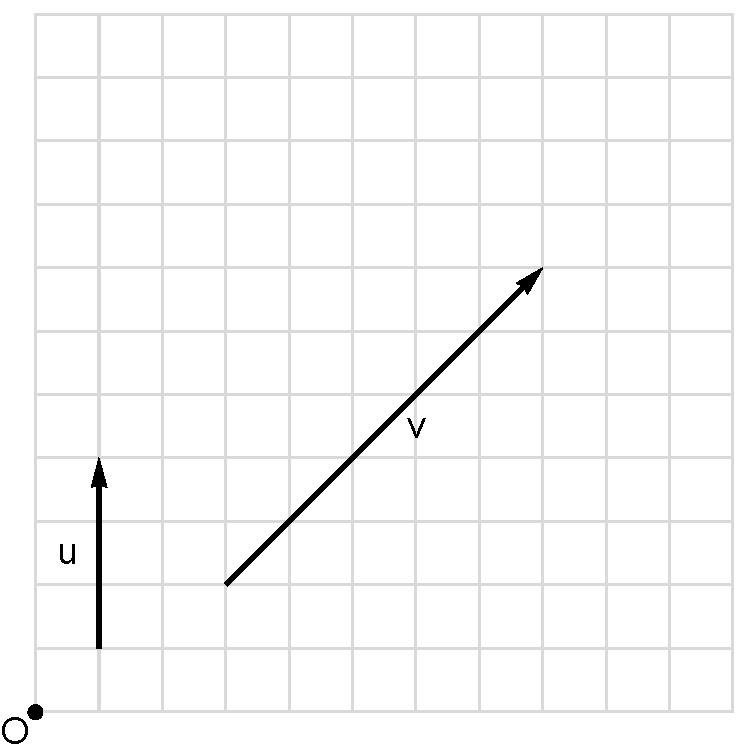
\includegraphics[scale=0.625]{img1}
		\end{center}
		\vspace{-0.4in}
		\item What are the lengths of $\vec{u}$ and $\vec{v}$? 
		\item Let $|\vec{w}|$ denote the length of an arbitrary vector $\vec{w}$. Is it true that $|\vec{u}|+|\vec{v}|=|\vec{u+v}|$?
		\item Write the coordinates of the \ti{terminal points} (i.e. the points in $\Reals^2$ where the arrowheads are located) for the translates of the vectors $\vec{u}$ and $\vec{v}$ which start at the origin $O$.
		\item Let $\vec{w}=\langle 5,11\rangle$. Show by means of a sketch that there are \ti{scalars} (i.e. real numbers) $s$ and $t$ such that $\vec{w}=s\vec{u}+t\vec{v}$.
		\item Use part (d) to find the scalars $s$ and $t$ mentioned in part (e).%to show that $\vec{w}=2\vec{u}+\vec{v}$ (i.e. that $s=2$ and $t=1$ in part (e)).
	\end{enumerate}
\end{enumerate}
\end{document}